%@+leo-ver=4-thin
%@+node:paran.20140514103950.1918:@shadow theTool.tex
%@@color
%@@language latex

\chapter{Refactor categories tool}
%@<<tool desc>>
%@+node:paran.20140731173741.2006:<<tool desc>>
In order to prove that having individual refactored views would provide some useful results we created a refator categories tool. The refactor categories tool examines the differences between files and arranges them into a greater variety of categories than used by version control systems or merge and diff tools.  In addition to being able to detect instances of delete, insert and modify the refactor categories tool can also detect instances where the code has been relocated and to some extent renamed.  It also can differentiate between changes to comments, white-space and Java code. This means it can differentiate between instances where a change to a source file causes a change in the behaviour of the program and some instances where it does not. Although it does not detect more complex differences beyond this we intend to show that changes exist in real world software projects that have no impact on how the project behaviour.
%@nonl
%@-node:paran.20140731173741.2006:<<tool desc>>
%@nl

\section{What the tool does}
%@<<What the tool does>>
%@+node:paran.20140605081907.1971:<<What the tool does>>
%@+at
% answer what it does and how
%@-at
%@@c

%@<<detecting moves>>
%@+node:paran.20140606104644.2007:<<detecting moves>>
By checking to see if an insert at one point matches a delete at another point it is possible to detect to see if the code block has moved. In order to determine if the move is one that has no impact the matches are only counted if a match can be found within the same container.  Here, a container is an enclosing scope within the source code, such as a class or method. For example if a method has been shifted within the same class the program will still act the same.  If a method is moved from one class into an inner class there is no guaramtee that they will be evaluated to determine if there is a suitable match.  If a method is shifted from one class to an inner class however the programs behaviour could have changed.
%@nonl
%@-node:paran.20140606104644.2007:<<detecting moves>>
%@nl

%@<<detecting renames>>
%@+node:paran.20140606104644.2009:<<detecting renames>>
To a limited extent the refactor categories tool can also deal with renaming.
%@nonl
%@-node:paran.20140606104644.2009:<<detecting renames>>
%@nl

%@<<detecting comments>>
%@+node:paran.20140606104644.2011:<<detecting comments>>
The refactor categories tool first does a cursory examination of the text differences between two files. It then examines both the differences in executable Java code and the differences between comments and white-space. 
%@-node:paran.20140606104644.2011:<<detecting comments>>
%@nl

%@<<detecting whitespace>>
%@+node:paran.20140606104644.2012:<<detecting whitespace>>
The refactor categories tool first does a cursory examination of the text differences between two files. It then examines both the differences in executable Java code and the differences in white-space.
%@nonl
%@-node:paran.20140606104644.2012:<<detecting whitespace>>
%@nl

%@-node:paran.20140605081907.1971:<<What the tool does>>
%@nl

\section{Overview}
%@<<Overview>>
%@+node:paran.20140805175513.2154:<<Overview>>
The refactor categories tool analyses all the historical changes ever made on a software project by extracting successive revisions from a Git repository using JGit.
An ordinary text comparison is used as a starting point.  The algorithm used for the text comparison is the histogram LCS one normally used by JGit with white space ignored. The text comparison returns the minimal number of text changes in EditList object.  The information about each change that the EditList object retains are:

\begin{itemize}
  \item the starting line of the change for both revisions being compared
  \item The ending line of the change for both revisions 
  \item The type of change that is being made
\end{itemize}

The types of changes that are detected between two files are limited to inserts, deletes, and modifications. In order to expand this list we need more information.  We obtain information about the meaning of Java files by parsing both revisions we are comparing into an AST using JastAddJ. We then need to discover which AST node matches which change to the source code. 

Each of the AST nodes can contain information about the line of source the AST node starts and ends at.  Unlike the EditList object which we have previously discussed AST node can also hold the column that the AST node starts and ends at.  Using this positional information we can match the text based changes to a set of AST nodes.

There is likely to be AST nodes that are not included in any of the change sets and can be safely ignored. In order to find just AST nodes we are interested in we need to traverse the AST.  When we start at the root of the AST the start position for the root node is the first line and the first column. The end position for the root node is the last line and last column.  By examining the children of the root however we can determine which children contain all or part of a text based change.

\begin{figure}[h]
 \begin{center}
  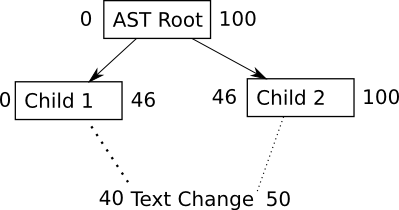
\includegraphics[scale=1]{DrilldownEx}
 \end{center}
 \caption{Finding an AST node we are interested in}
 \label{fig:findingASTNode}
\end{figure}  

An example of this can be found in figure \ref{fig:findingASTNode}.  In this figure it is safe to ignore any children of the AST node marked 'Child 1' because 'Child 1' does not contain the text change.  The AST Node marked 'Child 3' however is interesting as its location places it within a text change. 

In some instances items within the text change will not have a corresponding AST node.  These are of interest to us because these are instances where the text may have been changed but it has no impact on the behaviour of the program.  The most likely instances of this is when a comment has changed or if white space has been introduced in the middle of source code.Once the AST node for both revisions has been matched with the text change we can compare the AST nodes and their children to discover if they would behave in the same fashion. If they do behave in the same fashion it could indicate that the change is an astetic one.   

Another change we are interested in is if items have been moved.  We would notice this if there is a both insert and a delete for similar AST node types within the same scope.  If a method has been shifted within a class we would notice similar AST nodes, one being deleted at one location, the other being inserted at a different location.  This is another example of a text based change that does not change the behaviour of the program.

If we can keep track of renaming 

If we find examples of text based changes that do not change the programs behaviour we have an indication that we can reduce the amount of changes necesary to update another branch. This in turn could indicate that we would have less merge conflicts by reducing the overall number of changes.
%@-node:paran.20140805175513.2154:<<Overview>>
%@nl

\section{Performance}
%@<<Performance>>
%@+node:paran.20140805175513.2166:<<Performance>>
As we are testing the complete revision history for several projects there is a high number of changes.  This means that perfomance is an issue especally for large software projects that have many changes. This means we have not only had to look at using more memory for the refactor categories tool but also had to make some changes to the code to free up more memory where required.  

\begin{description}

  \item [By not analying AST node that did not have a text based change] 
  %@  <<not analysing>>
  %@+node:paran.20140805192059.2163:<<not analysing>>
  i.e the drill down speeds up performanace as you only need to analyase
  %@nonl
  %@-node:paran.20140805192059.2163:<<not analysing>>
  %@nl
  \item [By comparing only succsseive changes] 
  %@  <<successive changes>>
  %@+node:paran.20140805192059.2164:<<successive changes>>
  There are a greater amount of changes if we compare the head against a very old revision. By checking against successive we reduce the number of changes. This also could mean that we need to parse less files.
  %@nonl
  %@-node:paran.20140805192059.2164:<<successive changes>>
  %@nl
  \item [matching within only the required scope]  
  %@  <<matching within only the required scope>>
  %@+node:paran.20140805192059.2165:<<matching within only the required scope>>
  If we were not testing for moves in the same scope we would need to test every deleted AST node against every inserted AST node for the entire file. By stipulating that we can only be sure if it is a legal move if it is in the same scope we not only eliminate a lot of relocations of source code that are illegal but also reduce the number of items that need to be compared. In addition to this the AST node along with its type are recorded in a hashMap.  This ensures that only AST nodes that are a similar type are compared against each other
  %@nonl
  %@-node:paran.20140805192059.2165:<<matching within only the required scope>>
  %@nl
  
\end{description}

%@+at
% 
% removing the asts once they have been used
% 
% future work: by keeping track of equilvalencies there is no need to retest 
% using the AST
% 
%@-at
%@@c
%@nonl
%@-node:paran.20140805175513.2166:<<Performance>>
%@nl

\section{Design decisions}
%@<<design decisons>>
%@+node:paran.20140605081907.1972:<<design decisons>>
%@+at 
% 3) Add Section 4.4, called "Design Decision" where you discuss some of the 
% things you have at the beginning of your current Section 4.2.
% 
%@-at
%@@c

%@+at
% insert diagram of how it finds the ASTs that are within the change set
% 
% they are not associated with the AST changes because a comment could be at
% the end of a line and thus associated with the change before.  A multi-line
% comment is normally about the line that follows
%@-at
%@@c  

%@<<compares changes>>
%@+node:paran.20140801074838.2011:<<compares changes>>
There are a number of design differences between JDime and the refactor categories tool.  Instead of doing a text comparison first and only proceeding to analyse the program using an AST if there are conflicts the categorisation tool examines all files that have a difference in them.  Although this takes longer and is more memory intensive there are some advantages to this. The main advantage is related to the concept of keeping branches as consistent as possible whenever there is a change. An example of this advantage is if a merge was done using an ordinary text comparison and there is a non functional change to only one revision. Examples of a non functional change could include reordering methods or inserting a comment.  As the changes were only done to one of the revisions there is no conflict and JDime only does a text based merge.  During this text based merge, in addition to any of the changes to functionality that we want, we get the non functional changes that change the source code without changing the programs' behaviour. By examining all changes irrespective of if the text has conflicts means that the refactor categories tool can determine if it is a change that would not affect the behaviour of a program.
%@nonl
%@-node:paran.20140801074838.2011:<<compares changes>>
%@nl

%@<<drilldown>>
%@+node:paran.20140606104644.2019:<<drilldown>>
As there is a cost overhead with testing all the changes rather than just the conflicting ones the categorisation tool needs to be efficient in how it tests changes.  Assuming that changes occur in select areas within the file there are portions of the file that have not been changed.  We have developed a method that spends a smaller amount time in  within the portions that have already been identified as not containing changes.  Like JDime we initially do a text based merge.  The text based merge we use however uses the histogram merge in JGit.  This allows us to use information from the text based merge when we analyse the AST tree.  The information used is the ranges of line numbers and operations identified by the histogram merge. The change set has been taken from the original JGit based diff contains the start and end of the change in both files and what type of change it is (insert delete or modify).  By reusing these ranges of line numbers it is possible to figure out which AST items these changes affect. This is done by loading the file into the JastAddJ parser to get an AST tree. Line numbers for each item in the tree are then compared to line numbers from the change set. The line numbers are matched to the position information stored in each AST node using the following method.

The root of the AST is identified as the AST node we need to start at. 
We only begin any analysis, if the AST node resides completely within a block of text changes.
If there are any separate blocks of changes that occur between the start position of the AST node and the end position of the AST node then we recursively examine the AST nodes children.

%@+at
% The refactor categories tool first works out which text has changed using 
% the same method as JGit.
% This initial examination returns the differences based on a line by line 
% basis rather than using a smaller granularity.
% This means that the set of changes found could still contain code that is 
% comparatively the same.
% The set of changes found in using the JGit histogram comparison are then 
% evaluated.
% The reason for this is that some items of text could be in a differing order 
% but still be a valid Java program
% 
% 
% In order to resolve some limitations with JDime and the text only merge in 
% GIT information about which line numbers are retained after the first text 
% merge.  In JDime these are ignored and the AST is relied upon to hold all 
% the information.
%@-at
%@@c


%@+at
% after finished drill down we have a record of the same changes as JGit
% except now we also have the ASTs
%@-at
%@@c 
%@nonl
%@-node:paran.20140606104644.2019:<<drilldown>>
%@nl

%@<<resolving gaps>>
%@+node:paran.20140801202652.2011:<<resolving gaps>>
In some instances there is no position information stored in the JastAddJ AST nodes.  This could be because they are generated by the parser to reflect parts of the Java language that are inferred rather than directly mentioned in the code.  An example of this would be the use of super in the constructor.  Even if it is not written in the code for every constructor has a super. Likewise all methods mentioned in an interface have a public type even if is not in the code.

To get around this problem we have needed to discover the end position of the previous AST Node to determine the position the inferred AST node should occupy.  This means that the inferred AST node is in the right position but is not represented by a block of text in the source code. 
%@nonl
%@-node:paran.20140801202652.2011:<<resolving gaps>>
%@nl

%@+at 
% need to add something about the choice of java and jastaddj
%@-at
%@@c

%@<<comments and white space>>
%@+node:paran.20140606104644.2018:<<comments and white space>>
Comment and white-space are also examined separately as they also could give some indication of where code has been moved from or to.
Before being checked to find matches unnecessary white-space is identified and recorded.
Any text that remains is examined to determine if its is a comment. 

Because of the way we are using the position in the code to identify AST nodes there are circumstances when parts of the Java programming language are identified as being surplus text. These have already been identified and represented as an AST Node. By identifying comments we can eliminate any of the items falsely recorded as comments.

%@+at 
% Comments and white-space cannot be shown in the AST tree so they need to be
% dealt with separately
%@-at
%@@c
%@nonl
%@-node:paran.20140606104644.2018:<<comments and white space>>
%@nl

%@<<matcher>>
%@+node:paran.20140606104644.2016:<<matcher>>
%@+at
% comparing AST nodes
% the matcher and how using a score works
% finding the best match
% 
% 
% explain how we limit matching just to the parent of the thing being matched
%@-at
%@@c

Rather than comparing everything with each other to determine matches it is more efficient to match just the items that are under the same AST structure.  This means that it is more likely that we get a match that is going to be relevant and valid.  An example of this is matching methods. If the methods are under the same container (a class) they may be legally swapped without causing issues.  If the method has been moved to an inner class from an outer one however it becomes more complicated and we cannot guarantee that the code is equivalent.  
%@nonl
%@-node:paran.20140606104644.2016:<<matcher>>
%@nl

%@+at
% why does it do it for the whole repository
%@-at
%@@c

%@+at
% 
% note: we might want to use some literate programming here11
%@-at
%@@c
%@nonl
%@-node:paran.20140605081907.1972:<<design decisons>>
%@nl

\section{Limitations of the tool}
%@<<limitations>>
%@+node:paran.20140605081907.1993:<<limitations>>
The refactor categories tool focuses only on areas where there has been a change in the source code. 
It is harder to investigate any change that has causes side effects in unchanged code.  Fortunately it is not often that this type of side effect will be purposely placed in the code as it reflects bad design decisions.  This may however be an issue with bugs, which are unintentionally placed in the code.  
This also means that the refactor categories tool will not be able to tell when some code has been copied but the original remains unchanged. Instead it will assume that it is a completely new insertion of code.
%@-node:paran.20140605081907.1993:<<limitations>>
%@nl
%@-node:paran.20140514103950.1918:@shadow theTool.tex
%@-leo
